\chapter{Réalisation}
%%%%%%%%%%%%%%%%%%%%%%%%%%%%%%%%%%%%%%%%%%%%%%%%%
\section*{Introduction}
Tenant compte des besoins fixés et des choix conceptuels effectués, nous consacrons
ce chapitre à l’exposition du travail réalisé. Nous commençons par la description de
l’environnement matériel et logiciel utilisés. Nous terminons par des captures d’écrans traduisant le déroulement du projet et présentant les fonctionnalités développées.
%Pour finaliser notre projet, nous entamons la partie réalisation qui présente une importance, tant pour nous que pour la société concernée. Nous commençons par argumenter les choix matériel et logiciel, en présentant l’architecture du système ainsi que les technologies utilisées pour l’implémentation. Enfin, nous passons à la présentation de l’application par l’élaboration des captures d’écrans produites.
%%%%%%%%%%%%%%%%%%%%%%%%%%%%%%%%%%%%%%%%%%%%%%%%%
\section{Environnement de travail}
Dans ce paragraphe, nous présentons les outils matériels et logiciels adoptés pour l’achèvement de notre projet.
\subsection{Environnement matériel}
Notre application a été réalisée sur un ordinateur ayant les caractéristiques suivantes : 
\begin{itemize}
    \item Un processeur Intel(R) Core(TM) i5-5200U CPU @ 2.20GHz 2.20 GHz.
    \item Une mémoire RAM de 12 Go.
    \item Un disque dur de 1 To.
    \item Un système d'exploitation Windows 10.
\end{itemize}
%%%%%%%%%%%%%%%%%%%%%%%%%%%%%%%%%%%%%%%%%%%%%%%%%
\subsection{Environnement logiciel}
Dans cette partie, nous présentons les différents logiciels et outils utilisés:
\begin{itemize}
    \item \textbf{StarUML} \\
    C'est un logiciel de modélisation UML qui gère la plupart des diagrammes spécifiés dans la norme UML 2.0.
    \item \textbf{PostgreSQL}\\
    C'est un puissant système de gestion de bases de données open source. PostgreSQL fonctionne sur tous les principaux systèmes d'exploitation.
    \item \textbf{Intellij IDEA}\\
    C'est un environnement de développement intégré de technologie Java. Il est destiné au développement de logiciels informatiques.
    \item \textbf{Visual Studio Code}\\
    C'est un éditeur de code source, léger mais puissant. Il dispose d'un riche écosystème d'extensions pour d'autres langages (tels que C ++, C\#, Java, Python, PHP, Go).
    \item \textbf{Docker}\\
    C'est un logiciel libre permettant de lancer des applications dans des conteneurs logiciels. Un conteneur est une unité logicielle standard qui regroupe le code et toutes ses dépendances, et qui permet à l'application de s'exécuter rapidement et de manière fiable, d'un environnement informatique à un autre.
    \item \textbf{Overleaf}\\
    C'est un éditeur LaTeX en ligne, collaboratif en temps réel. Il est utilisé pour la rédaction, l'édition et la publication de documents scientifiques.
\end{itemize}
%%%%%%%%%%%%%%%%%%%%%%%%%%%%%%%%%%%%%%%%%%%%%%%%%
\subsection{Technologies utilisées}
Dans cette partie, nous nous intéressons aux langages et aux bibliothèques utilisés tout au long de la réalisation de notre application tout en justifiant notre choix.
\begin{itemize}
    \item \textbf{Spring Boot}\\
    C'est un framework de développement applicatif JAVA open Source. Il est particulièrement recommandé pour le développement des microservices. Ses points forts sont l'auto-configuration ainsi que les annotations.
    \item \textbf{Spring Cloud Eureka Client}\\
    Il permet aux différents microservices de s'enregistrer dans l'annuaire des services Eureka. La Figure \ref{fig:capture_eureka} montre la liste des microservices détectés par le service Eureka. 
    \begin{figure}[H]
     \centering
     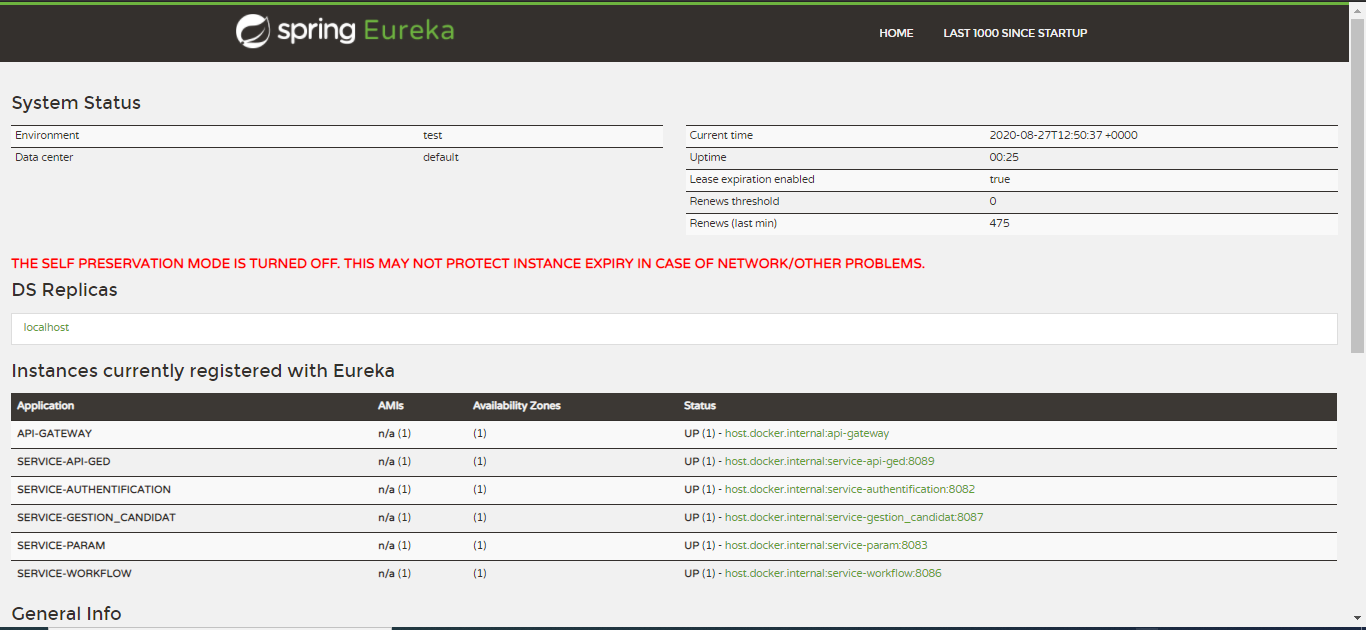
\includegraphics[scale=0.47]{img/capture eureka.PNG}
     \caption{Interface de Eureka Discovery Service}
     \label{fig:capture_eureka}
 \end{figure}
    \item \textbf{Spring Data JPA}\\
    Il vise à améliorer d'une manière significative la mise en oeuvre des couches d'accès aux données en réduisant la quantité de code à écrire.
    \item \textbf{QueryDsl}\\
    C'est un framework qui permet la construction des requêtes SQL typées dynamiquement via son API fluide.
    \item \textbf{Angular 7}\\
    C'est framework JavaScript libre, développé par Google et utilisé pour créer des applications Web basées sur une seule page (Single Page Application). Il utilise des fonctionnalités de plate-forme Web modernes pour offrir de nouvelles expériences, ayant une installation à haute performance avec zéro-étape.
\end{itemize}
%%%%%%%%%%%%%%%%%%%%%%%%%%%%%%%%%%%%%%%%%%%%%%%%%
\section{Les interfaces utilisateur}
Nous exposerons dans cette section les interfaces homme-machine qui sont un élément important pour la réussite d'une application.
%%%%%%%%%%%%%%%%%%%%%%%%%%%%%%%%%%%%%%%%%%%%%%%%%
\subsection{Interface d'authentification}
Pour pouvoir accéder aux différentes fonctionnalités de l’application, l'utilisateur doit saisir son login et son mot de passe comme le montre la Figure \ref{fig:capture_auth}.
\begin{figure}[H]
     \centering
     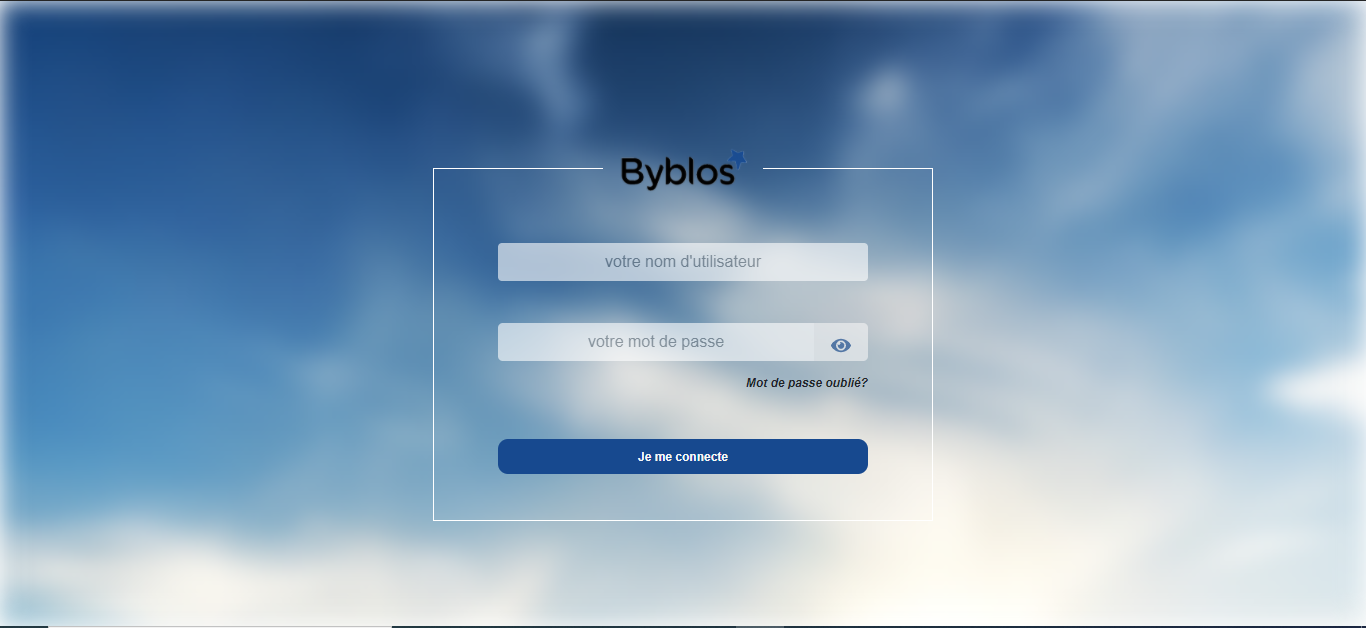
\includegraphics[scale=0.5]{img/capture authentification.PNG}
     \caption{Interface d'authentification}
     \label{fig:capture_auth}
 \end{figure}
%%%%%%%%%%%%%%%%%%%%%%%%%%%%%%%%%%%%%%%%%%%%%%%%%%%
\subsection{Interface d'accueil}
Après l'authentification de l'utilisateur, la page d'accueil est chargée comme le montre la Figure \ref{fig:capture_accueil}. Elle contient le KPI des avis des entretiens composé des éléments suivants :
\begin{itemize}
    \item Une liste prédéfinie des avis distingués par des couleurs différentes.
    \item Un graphe en secteurs de différentes couleurs. Chaque secteur contient le nombre total de candidats correspondant à un avis donné.
    \item L'année choisie ainsi que deux boutons pour sélectionner l'année suivante ou bien l'année précédente.
    \item Deux boutons en bas, l'un dirige vers une nouvelle fiche candidat, l'autre vers l'interface de recherche de candidats.  
    
\end{itemize}
 
\begin{figure}[H]
     \centering
     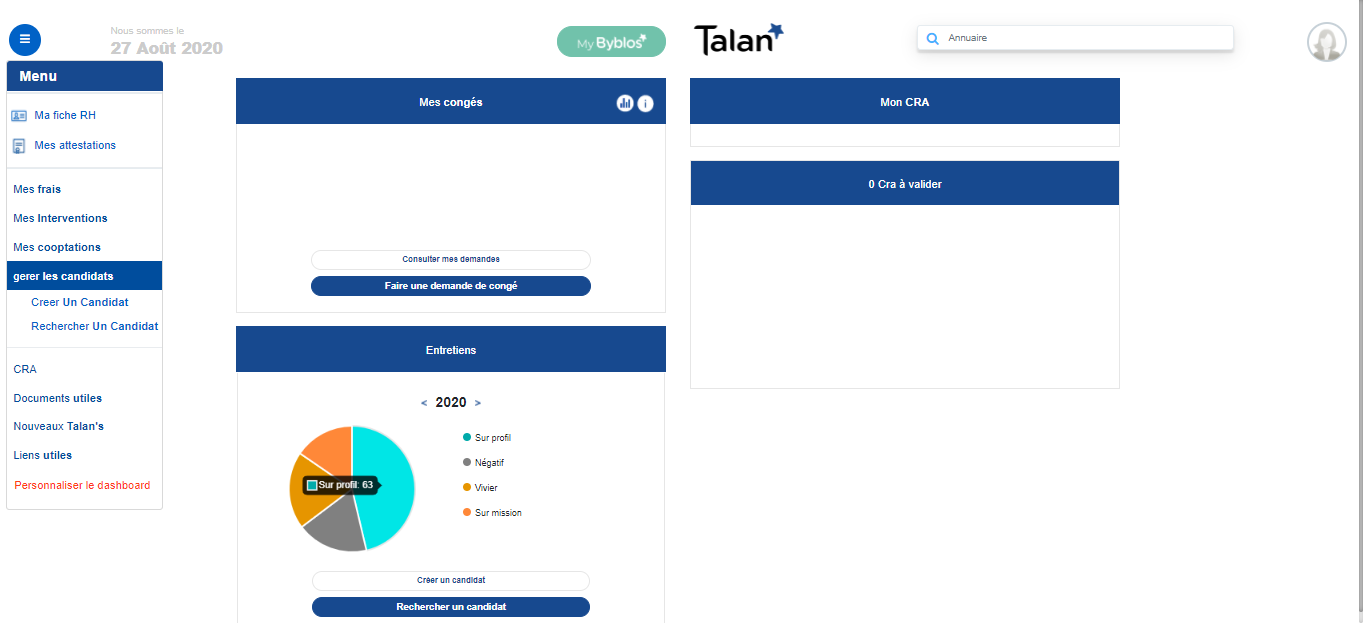
\includegraphics[scale=0.5]{img/capture accueil 2.png}
     \caption{Interface d'accueil}
     \label{fig:capture_accueil}
 \end{figure}
%%%%%%%%%%%%%%%%%%%%%%%%%%%%%%%%%%%%%%%%%%%%%%%%%%%
\subsection{Interface d'ajout d'une fiche candidat}
Cette interface est composée de trois parties :
\begin{enumerate}[label=\textbf{\arabic*. }]
    \item \textbf{Fiche candidat} : elle contient les informations qui concernent le candidat. Cette partie se compose de quatre formulaires listés ci-dessous :
    \begin{enumerate}
        \item [•] \textbf{Interface identité:} \\Cette interface, représentée dans la Figure \ref{fig:capture_fiche_identité}, contient les informations liées à l'identité du candidat: son nom, son prénom, sa date de naissance $\dots$ 
         \begin{figure}[H]
     \centering
     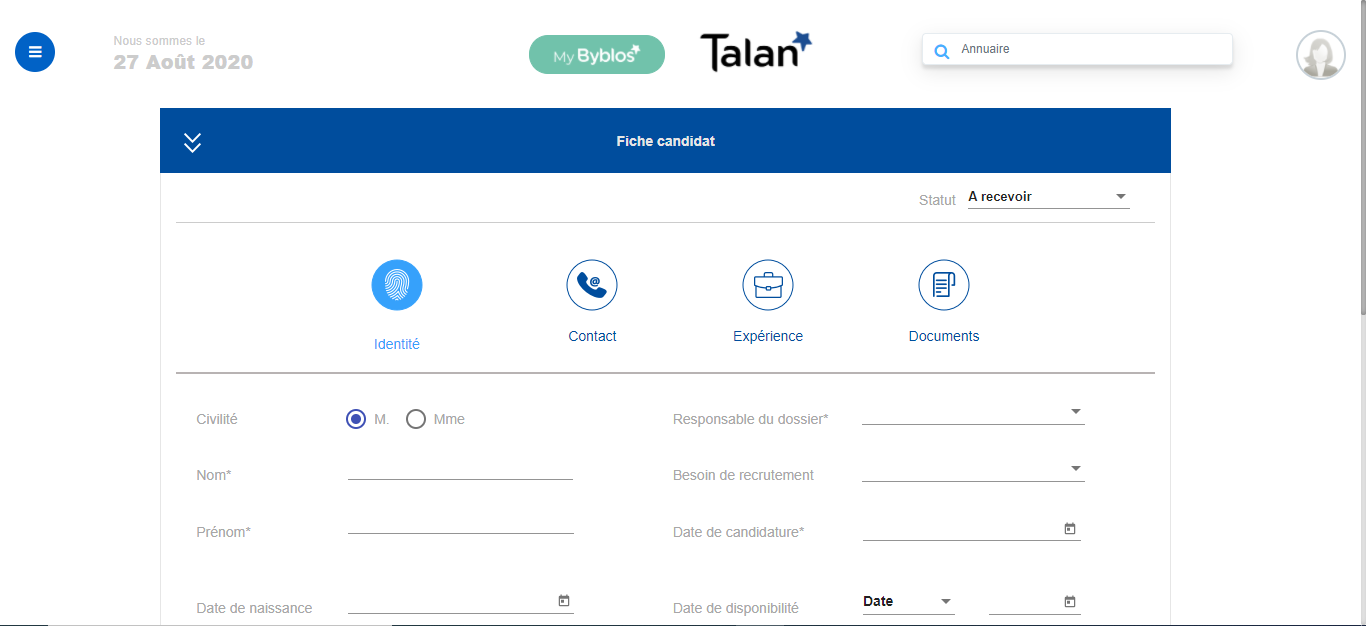
\includegraphics[scale=0.5]{img/capture fiche candidat identite.PNG}
     \caption{Interface Identité}
     \label{fig:capture_fiche_identité}
 \end{figure}
    \end{enumerate}
    \item [•] \textbf{Interface contact:}\\Cette interface, représentée dans la Figure \ref{fig:capture_fiche_contact}, contient les coordonnées du candidat: son numéro du téléphone et son e-mail.
    \begin{figure}[H]
     \centering
     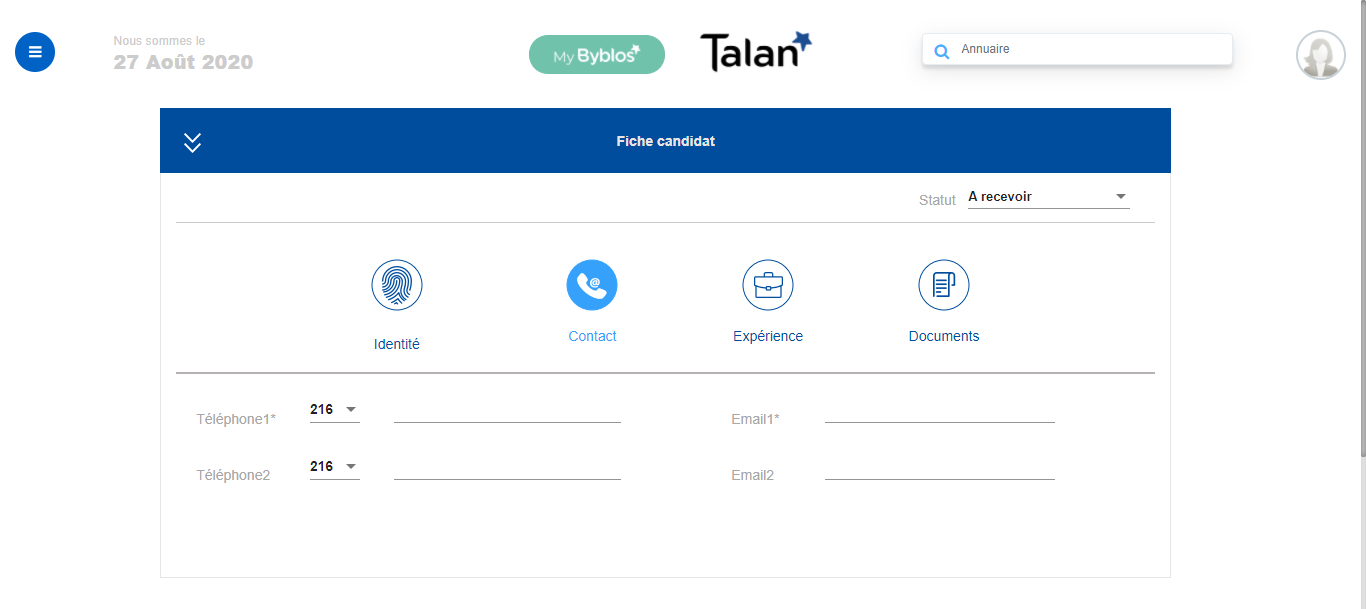
\includegraphics[scale=0.5]{img/capture fiche candidat contact.PNG}
     \caption{Interface Contact}
     \label{fig:capture_fiche_contact}
 \end{figure}
    \item [•] \textbf{Interface expérience:}\\ Cette interface, représentée dans la Figure \ref{fig:capture_fiche_experience}, contient les informations concernant l'expérience professionnelle du candidat.  
     \begin{figure}[H]
     \centering
     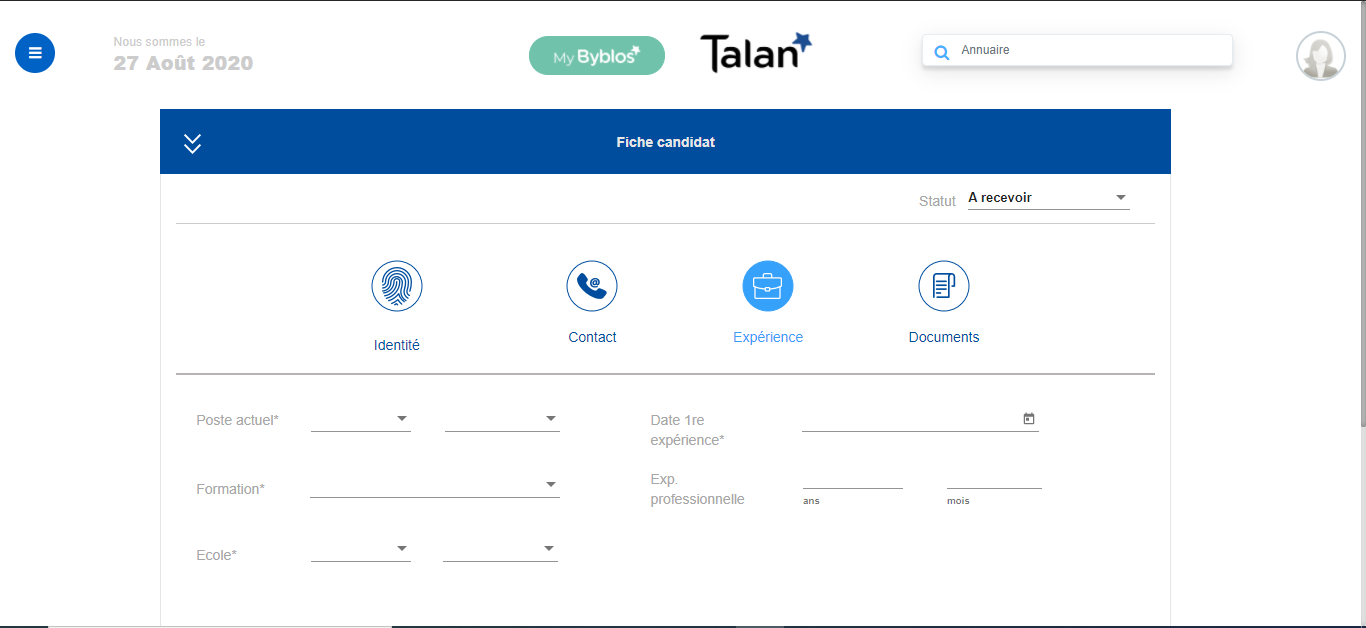
\includegraphics[scale=0.5]{img/capture fiche candidat experience.PNG}
     \caption{Interface Expérience}
     \label{fig:capture_fiche_experience}
 \end{figure}
    \item [•] \textbf{Interface Documents:}\\ Cette interface, représentée dans la Figure \ref{fig:capture_fiche_documents}, contient les informations concernant la pièce d'identité du candidat ainsi que son CV.
     \begin{figure}[H]
     \centering
     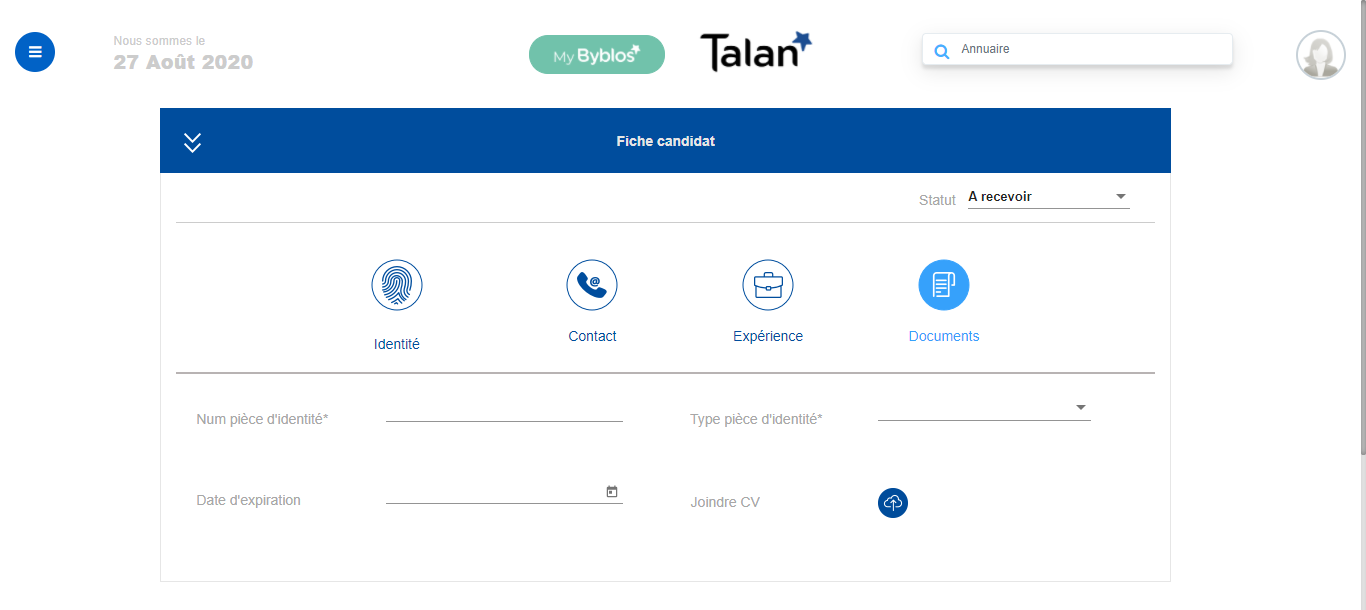
\includegraphics[scale=0.5]{img/capture fiche candidat Documents.PNG}
     \caption{Interface Documents}
     \label{fig:capture_fiche_documents}
 \end{figure}
\item \textbf{Planification des entretiens:}\\ Cette interface, représentée dans la Figure \ref{fig:capture_planifier_entretiens}, contient la liste des entretiens déjà planifiés, avec un bouton permettant de planifier un nouvel entretien.
 \begin{figure}[H]
     \centering
     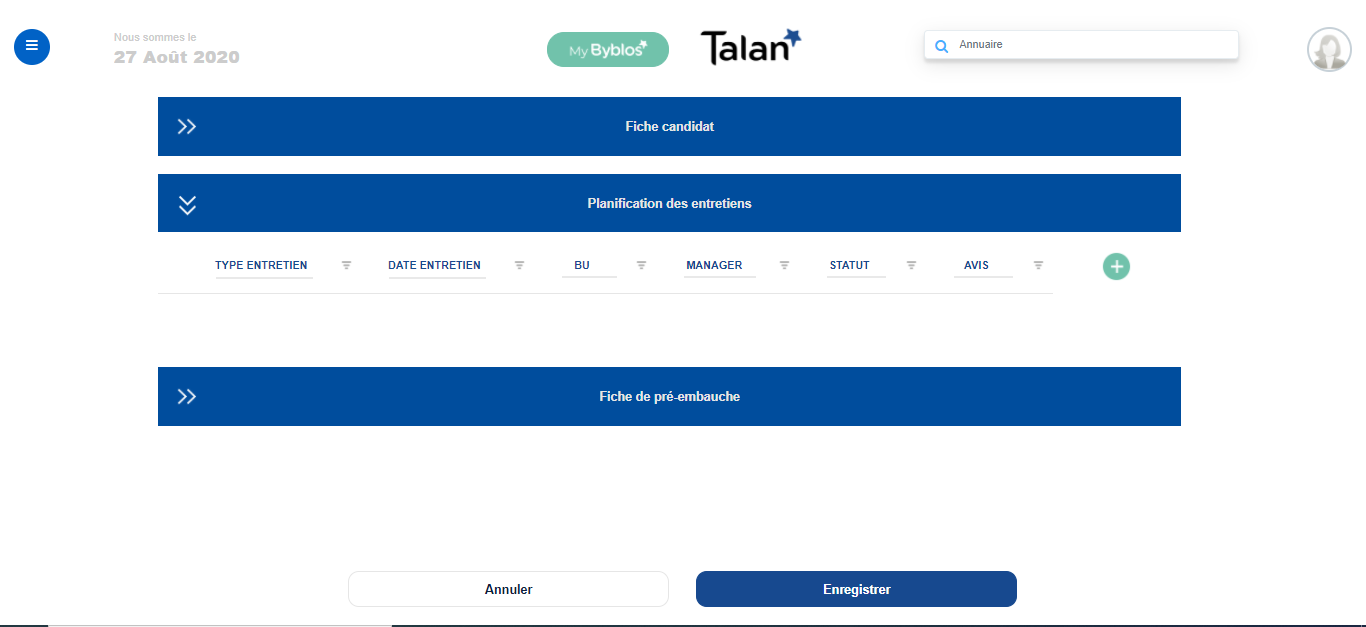
\includegraphics[scale=0.5]{img/capture fiche candidat 1.PNG}
     \caption{Interface Planification des entretiens}
     \label{fig:capture_planifier_entretiens}
 \end{figure}
\item \textbf{Fiche de pré-embauche}\\ Cette interface contient les informations concernant le contrat de pré-embauche à signer par le candidat s'il est accepté. Cette interface est composée de trois formulaires listés ci-dessous :
\begin{enumerate}
    \item [•] \textbf{Interface contrat} \\ Cette interface, représentée dans la Figure \ref{fig:capture_embauche_contrat}, contient les différentes informations contenues dans le contrat à signer.
    \begin{figure}[H]
     \centering
     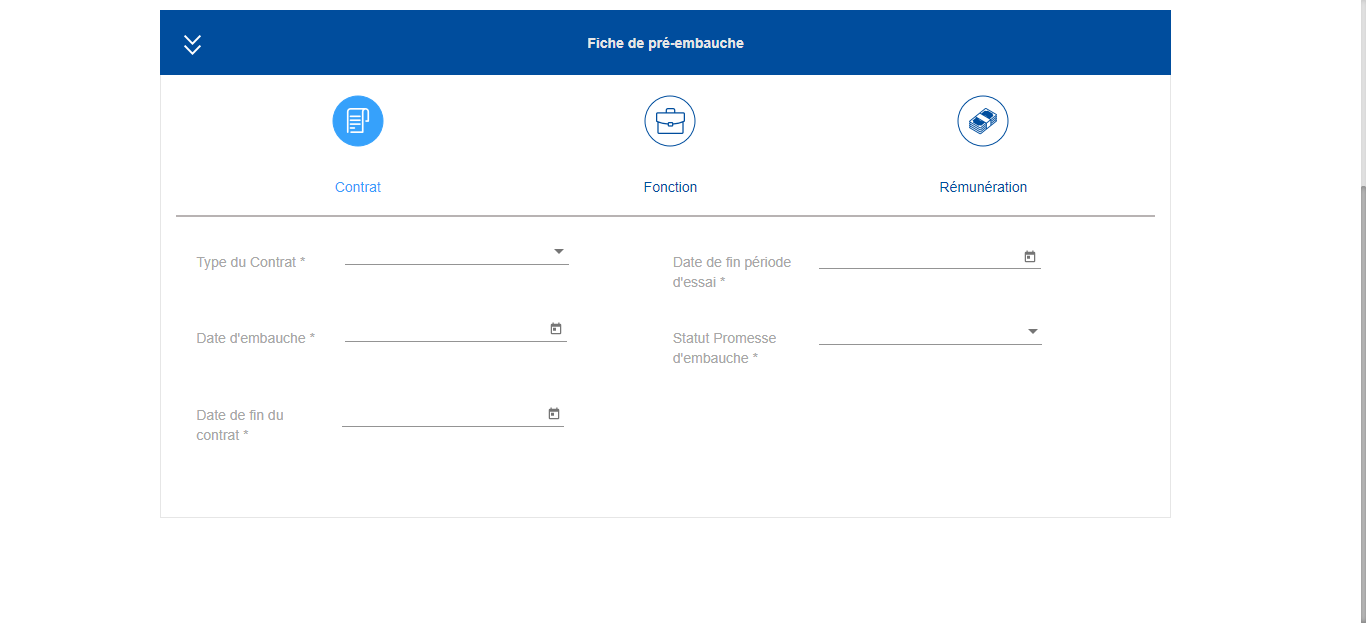
\includegraphics[scale=0.5]{img/capture fiche pre-embauche contrat.PNG}
     \caption{Interface Contrat}
     \label{fig:capture_embauche_contrat}
 \end{figure}
    \item [•] \textbf{Interface fonction} \\  Cette interface, représentée dans la Figure \ref{fig:capture_embauche_fonction}, contient les informations concernant la fonction que le candidat va occuper.
    \begin{figure}[H]
     \centering
     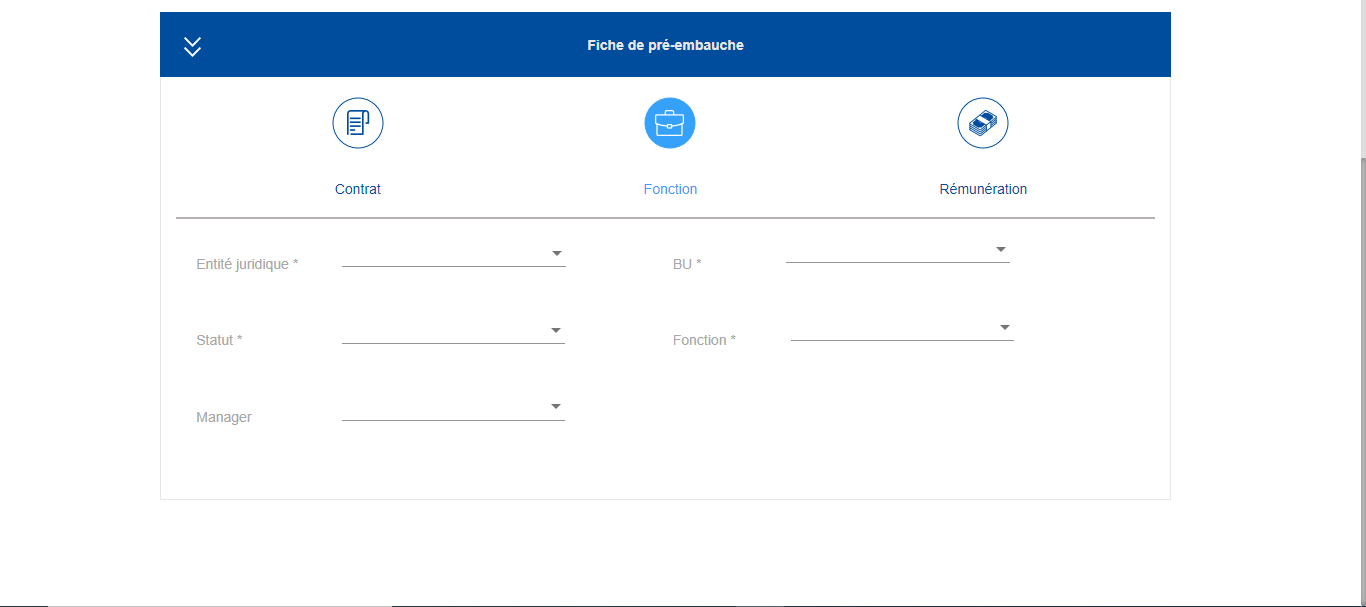
\includegraphics[scale=0.5]{img/capture fiche pre-embauche fonction.PNG}
     \caption{Interface Fonction}
     \label{fig:capture_embauche_fonction}
 \end{figure}
    \item [•] \textbf{Interface rémunération} \\ Cette interface, représentée dans la Figure \ref{fig:capture_embauche_remuneration}, contient les informations concernant la rémunération qui sera attribuée au candidat. 
    \begin{figure}[H]
     \centering
     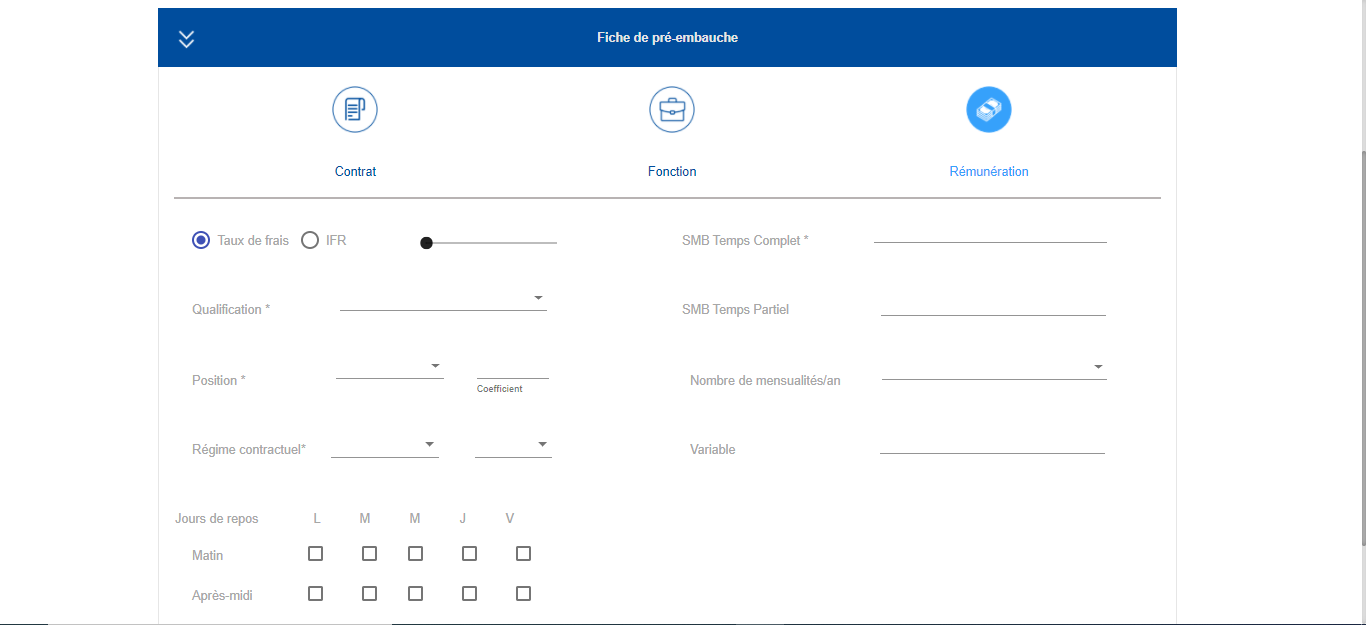
\includegraphics[scale=0.5]{img/capture fiche pre-embauche remuneration.PNG}
     \caption{Interface Rémunération}
     \label{fig:capture_embauche_remuneration}
 \end{figure}
\end{enumerate}
\end{enumerate}
%%%%%%%%%%%%%%%%%%%%%%%%%%%%%%%%%%%%%%%%%%%%%%%%%
\subsection{Interface de la recherche d'un candidat}
Cette interface, représentée dans la Figure \ref{fig:capture_recherche}, comporte un filtre contenant les critères de recherche sélectionnés, avec la possibilité d'omettre certains d'entre eux ainsi que le formulaire de recherche et un tableau contenant le résultat obtenu.
\begin{figure}[H]
     \centering
     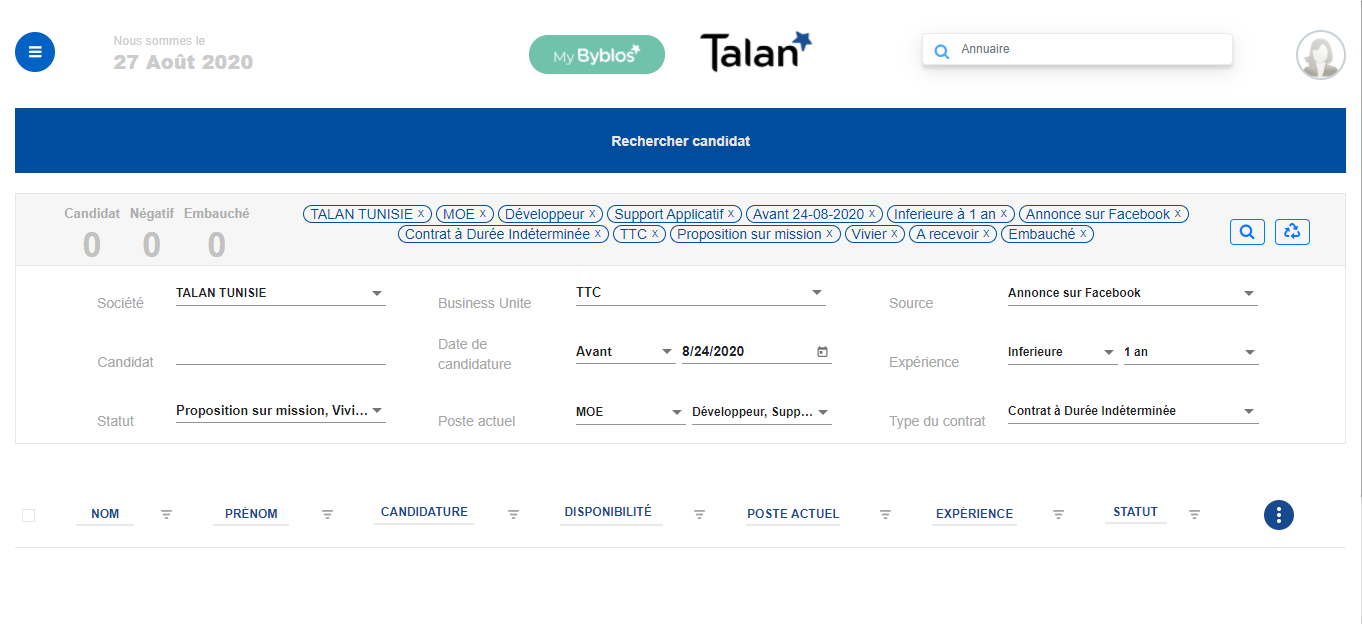
\includegraphics[scale=0.5]{img/capture recherche candidat.PNG}
     \caption{Interface de la recherche d'un candidat}
     \label{fig:capture_recherche}
 \end{figure}
 %%%%%%%%%%%%%%%%%%%%%%%%%%%%%%%%%%%%%%%%%%%%%%%%
 \subsection{Interface du résultat de la recherche}
 Cette interface, représentée dans la Figure \ref{fig:capture_resultat_recherche}, comporte une partie qui contient le nombre total de candidats répondant aux critères de la recherche effectuée, le nombre  de candidats ayant un statut "\textbf{Négatif}" et le nombre  de candidats ayant un statut "\textbf{Embauché}". Elle comporte aussi un tableau détaillant le résultat de la recherche, ainsi qu'un bouton permettant le téléchargement d'un fichier excel qui contient les candidats sélectionnés. 
 \begin{figure}[H]
     \centering
     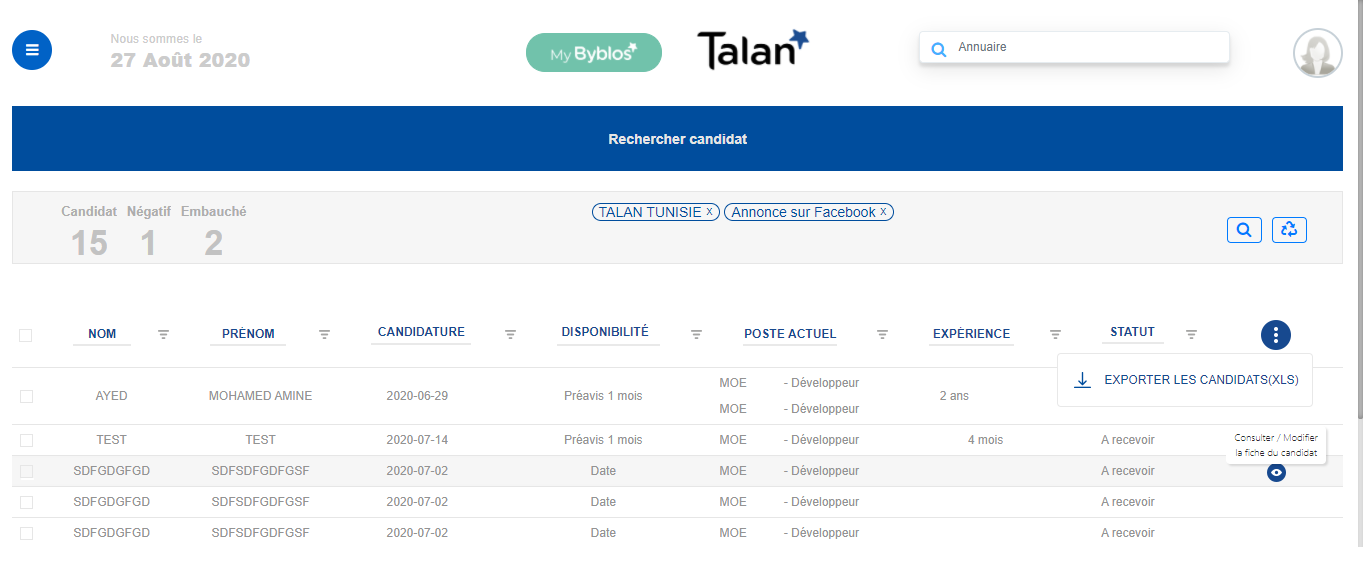
\includegraphics[scale=0.5]{img/capture resultat recherche.png}
     \caption{Interface du résultat de la recherche}
     \label{fig:capture_resultat_recherche}
 \end{figure}
 %%%%%%%%%%%%%%%%%%%%%%%%%%%%%%%%%%%%%%%%%%%%%%%%
 \subsection{Interface du fichier excel contenant le résultat de la recherche}
 Cette interface, représentée dans la Figure \ref{fig:capture_fichier_excel}, comporte le fichier excel téléchargé précédemment et qui contient les différentes informations concernant les candidats sélectionnés.  
 \begin{figure}[H]
     \centering
     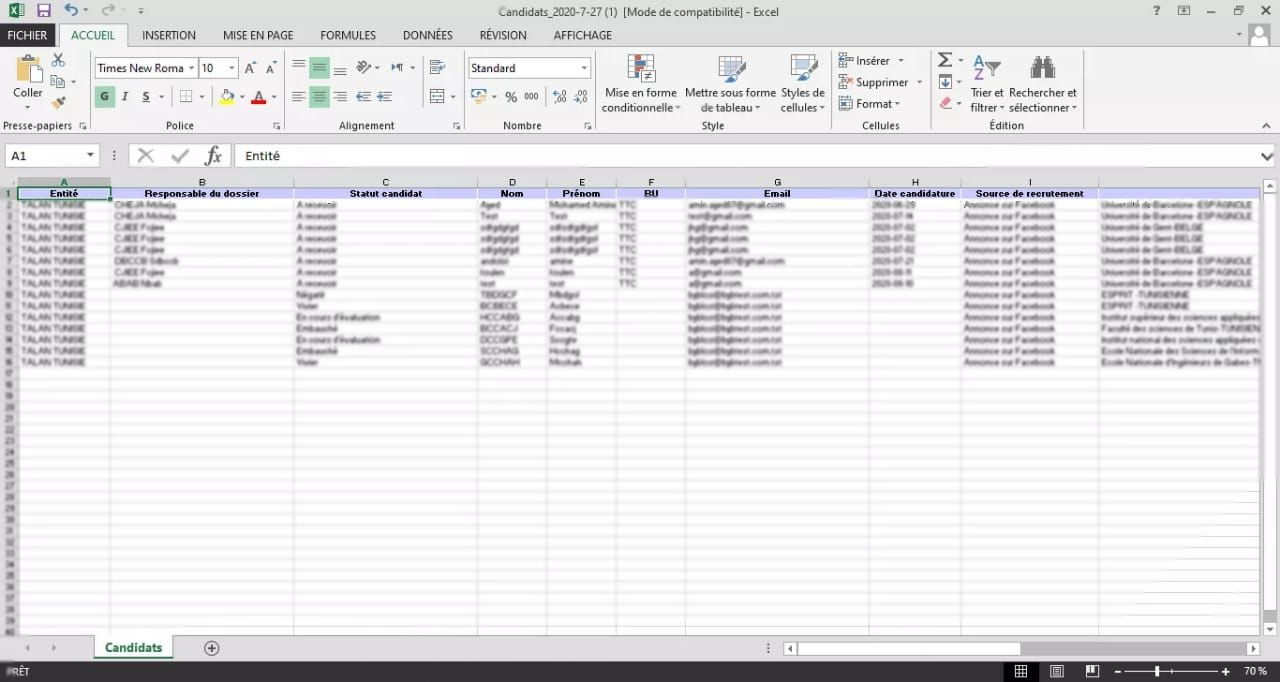
\includegraphics[scale=0.45,width=\textwidth]{img/WhatsApp Image 2020-08-27 at 17.09.20.jpeg}
     \caption{Interface du fichier excel contenant le résultat de recherche}
     \label{fig:capture_fichier_excel}
 \end{figure}
 %%%%%%%%%%%%%%%%%%%%%%%%%%%%%%%%%%%%%%%%%%%%%%%%
 \subsection{Interface de la planification d'un entretien}
 Cette interface, représentée dans la Figure \ref{fig:capture_planifier_entretien}, contient le formulaire utilisé pour planifier un nouvel entretien.
 \begin{figure}[H]
     \centering
     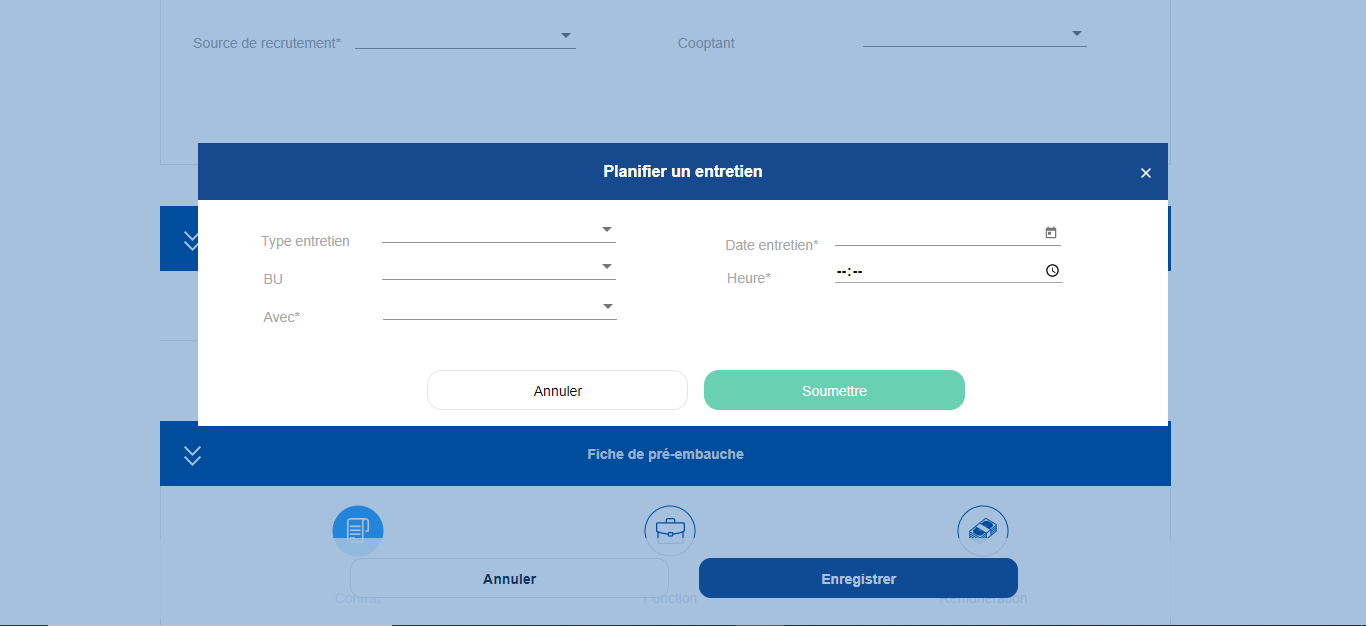
\includegraphics[scale=0.5]{img/capture planifier entretien.PNG}
     \caption{Interface de la planification d'un entretien}
     \label{fig:capture_planifier_entretien}
 \end{figure}
%%%%%%%%%%%%%%%%%%%%%%%%%%%%%%%%%%%%%%%%%%%%%%%%%
\subsection{Interface contenant l'e-mail de validation de l'entretien}
Cette interface, représentée dans la Figure \ref{fig:capture_email_validation}, contient l'e-mail envoyé au recruteur après la planification de l'entretien par le back-office, pour qu'il soit accepté ou refusé.
\begin{figure}[H]
     \centering
     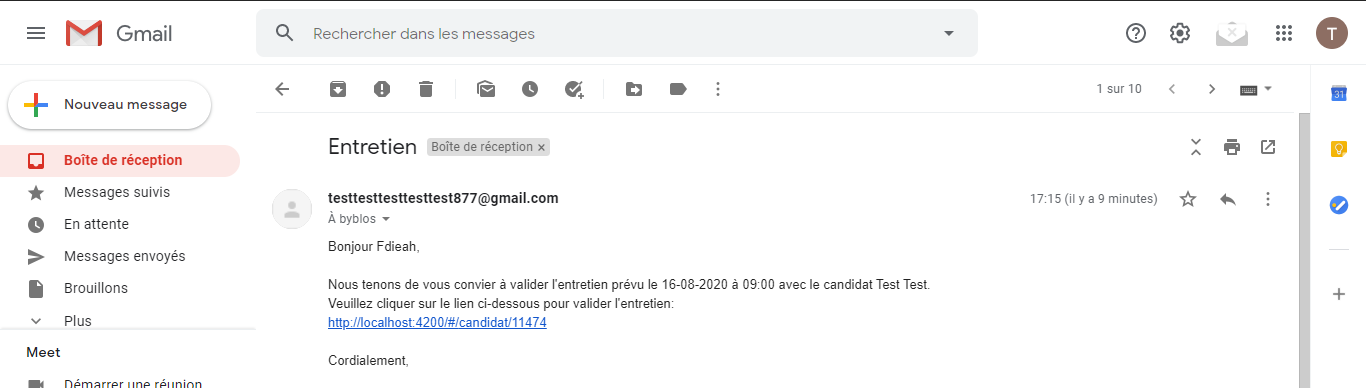
\includegraphics[scale=0.5]{img/capture mail de validation.PNG}
     \caption{Interface contenant l'e-mail de validation de l'entretien}
     \label{fig:capture_email_validation}
 \end{figure}
 %%%%%%%%%%%%%%%%%%%%%%%%%%%%%%%%%%%%%%%%%%%%%%%%
 \subsection{Interface contenant l'e-mail du rejet de l'entretien }
 Si le recruteur rejette l'entretien, un e-mail sera envoyé au back-office pour lui notifier ce refus. Cette interface est représentée dans la Figure \ref{fig:capture_email_rejet}.
 \begin{figure}[H]
     \centering
     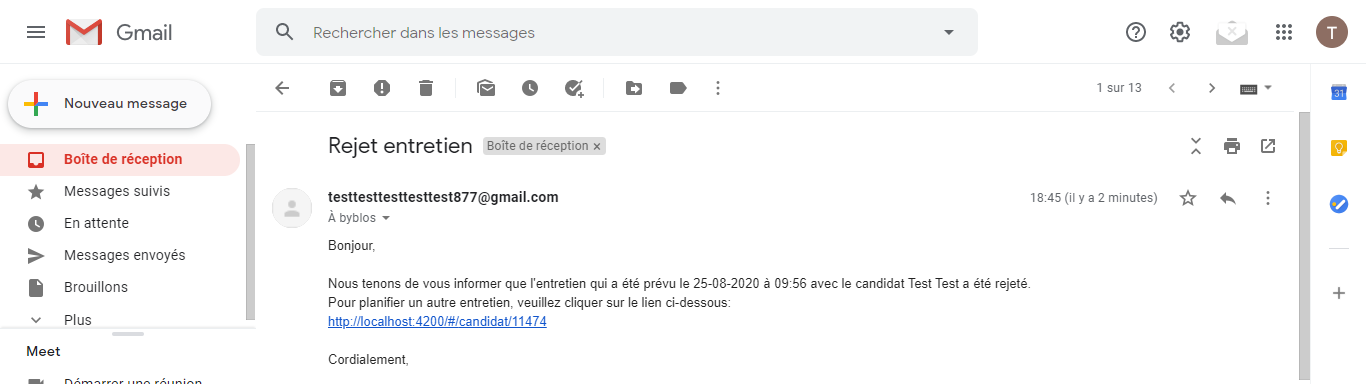
\includegraphics[scale=0.5]{img/capture mail rejet entretien.PNG}
     \caption{Interface contenant l'e-mail du rejet de l'entretien}
     \label{fig:capture_email_rejet}
 \end{figure}
 %%%%%%%%%%%%%%%%%%%%%%%%%%%%%%%%%%%%%%%%%%%%%%%%
\subsection{Interface contenant les différents statuts des entretiens}
Un entretien peut avoir l'un des statuts suivants :
\begin{itemize}
    \item "\textbf{Accepté}" : représenté sous forme d'une icône verte.
    \item "\textbf{Rejeté}" : représenté sous forme d'une icône rouge.
    \item "\textbf{En attente}" : représenté sous forme d'une icône bleue.
\end{itemize}
Cette interface est représentée dans la Figure \ref{fig:capture_liste_entretien}.
\begin{figure}[H]
     \centering
     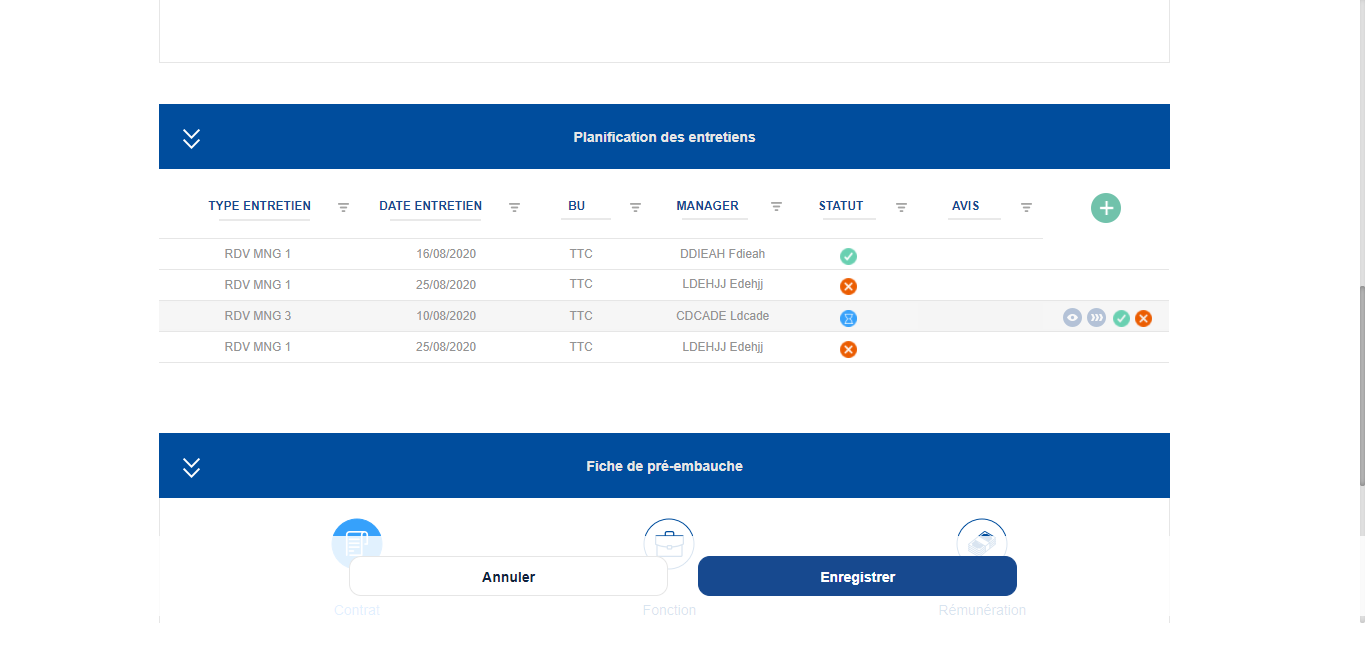
\includegraphics[scale=0.5]{img/cpature liste entretien.png}
     \caption{Interface contenant les différents statuts des entretiens}
     \label{fig:capture_liste_entretien}
 \end{figure}
%%%%%%%%%%%%%%%%%%%%%%%%%%%%%%%%%%%%%%%%%%%%%%%%%
\subsection{Interface de la consultation du Workflow d'un entretien en attente}
Cette interface, montrée dans la Figure \ref{fig:capture_entretien_en_attente}, représente le Workflow d'un entretien qui est en attente de validation par le recruteur.
\begin{figure}[H]
     \centering
     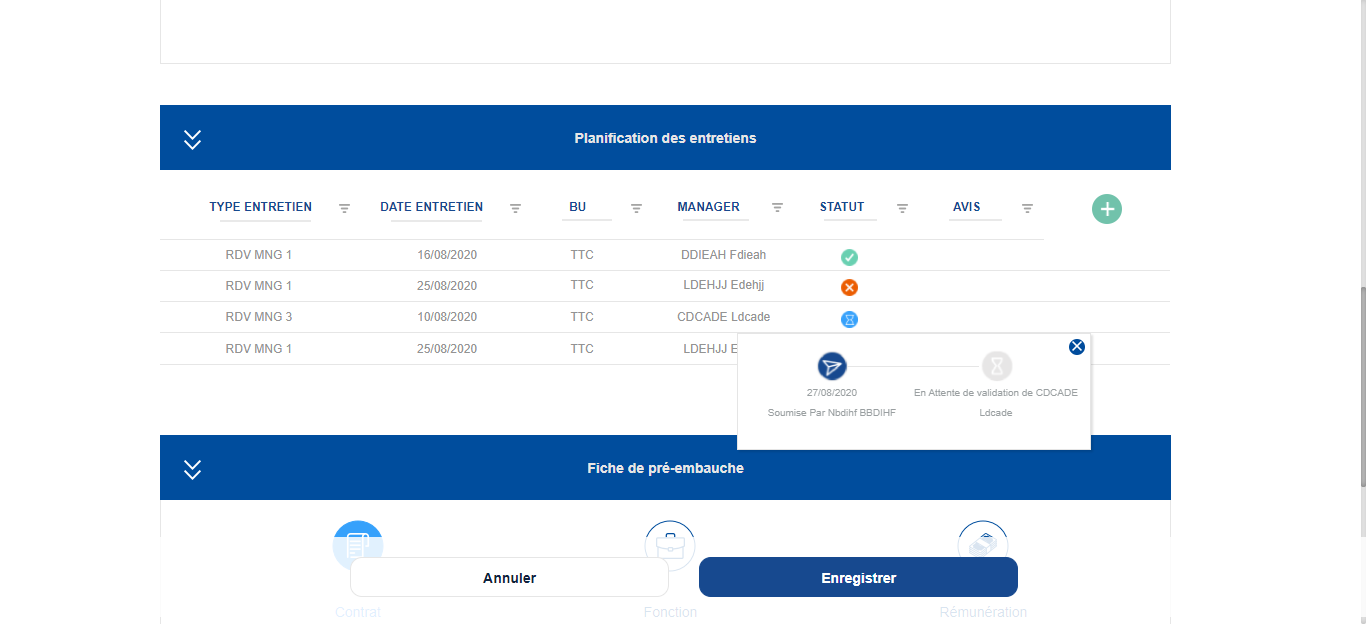
\includegraphics[scale=0.5]{img/capture entretien statut en attente.png}
     \caption{Interface de la consultation du Workflow d'un entretien en attente de validation}
     \label{fig:capture_entretien_en_attente}
 \end{figure}
 %%%%%%%%%%%%%%%%%%%%%%%%%%%%%%%%%%%%%%%%%%%%%%%%
\subsection{Interface de la consultation du Workflow d'un entretien accepté}
Cette interface, représentée dans la Figure  \ref{fig:capture_entretien_accepte}, montre le Workflow d'un entretien accepté.
\begin{figure}[H]
     \centering
     \includegraphics[scale=0.5]{img/capture entretien statut accepté.PNG}
     \caption{Interface de la consultation du Workflow d'un entretien accepté}
     \label{fig:capture_entretien_accepte}
 \end{figure}
 %%%%%%%%%%%%%%%%%%%%%%%%%%%%%%%%%%%%%%%%%%%%%%%%
\subsection{Interface de la consultation du Workflow d'un entretien rejeté}
Cette interface, représentée dans la Figure  \ref{fig:capture_entretien_rejeté}, montre le Workflow d'un entretien rejeté.
\begin{figure}[H]
     \centering
     \includegraphics[scale=0.5]{img/capture entretien statut refusé.PNG}
     \caption{Interface de la consultation du Workflow d'un entretien rejeté}
     \label{fig:capture_entretien_rejeté}
 \end{figure}
%%%%%%%%%%%%%%%%%%%%%%%%%%%%%%%%%%%%%%%%%%%%%%%%%
\section*{Conclusion}
La phase de réalisation est l’étape la plus exigeante en termes d'efforts et de temps. Elle nous a permis de concrétiser et d’approfondir nos connaissances académiques grâce à l’opportunité qui nous a été offerte pour la réalisation d’un projet informatique réel au sein
d’une grande entreprise. Ce chapitre constitue en fait l’aboutissement des phases précédentes. 
